% \documentclass[12pt,openright]{book}
% \usepackage{emptypage}
% \PassOptionsToPackage{a4paper, inner=3cm, outer=2cm, top=2.5cm, bottom=2.5cm}{geometry}

% \documentclass[12pt,openany]{book}
% \usepackage{emptypage}
% \PassOptionsToPackage{a4paper, inner=3cm, outer=2cm, top=2.5cm, bottom=2.5cm}{geometry}

% \documentclass[12pt,openright]{book}
% \PassOptionsToPackage{paperwidth=17cm, paperheight=25.7cm, margin=.5cm}{geometry}

\documentclass[12pt,openany]{book}
\PassOptionsToPackage{paperwidth=17cm, paperheight=25.7cm, margin=.5cm}{geometry}

\PassOptionsToPackage{english,main=indonesian}{babel}
\PassOptionsToPackage{autostyle}{csquotes}
\PassOptionsToPackage{hidelinks}{hyperref}
\PassOptionsToPackage{authoryear}{natbib}
\PassOptionsToPackage{table,xcdraw}{xcolor}

\usepackage{
	babel,
	csquotes,
	amsthm,
	lmodern,
	newtxtext,
	newtxmath,
	newtxtt,
	geometry,
	pagecolor,
	parskip,
	titlesec,
	array,
	multirow,
	float,
	graphicx,
	subcaption,
	xcolor,
	% pdflscape,
	lscape,
	hyperref,
	cleveref,
	natbib,
	fancyhdr,
	algorithm
}

\def\True{\mathtt{True}}
\def\False{\mathtt{False}}

\newcommand{\foreign}[1]{\foreignlanguage{english}{\textit{#1}}}

\theoremstyle{definition}
\newtheorem{examplex}{Contoh}

\newenvironment{example}
	{\begin{examplex}\pushQED{\qed}}
	{\popQED\end{examplex}}

\addto\extrasindonesian{
	\renewcommand{\chapterautorefname}{Bab}
	\renewcommand{\sectionautorefname}{Bagian}
	\renewcommand{\subsectionautorefname}{Subbagian}
	\renewcommand{\figureautorefname}{Gambar}
	\renewcommand{\tableautorefname}{Tabel}
	\renewcommand{\equationautorefname}{Persamaan}
	\floatname{algorithm}{Algoritma}
	\renewcommand{\refname}{Daftar Pustaka}
	\renewcommand{\bibname}{Daftar Pustaka}
	\providecommand{\algorithmautorefname}{Algoritma}
	\providecommand{\examplexautorefname}{Contoh}
	\crefname{appsec}{Lampiran}{Appendices}
	\Crefname{appsec}{Lampiran}{Appendices}
}

\newcommand{\bulan}[1]{
	\ifcase#1\relax
		\or Januari\or Februari\or Maret\or April\or Mei\or Juni\or Juli\or Agustus\or September\or Oktober\or Nopember\or Desember%
	\fi
}

\titleformat{\chapter}[display]
	{\centering\LARGE\bfseries}
	{\MakeUppercase{\chaptername~\Roman{chapter}}}
	{0pt}
	{\MakeUppercase}

\titlespacing*{\chapter}
	{0pt}
	{0pt}
	{2\parskip}

\raggedbottom

\pagestyle{fancy}
\fancyhf{}
\renewcommand{\headrulewidth}{0pt}
\fancyfoot[LE,RO]{\thepage}
\fancypagestyle{plain}{
	\fancyfoot[LE,RO]{\thepage}
}


\newcommand{\titleBahasa}{Menentukan Dimensi Metrik Menggunakan \foreign{Satisfiability Modulo Theories}}

\newcommand{\titleEnglish}{Determining Metric Dimension with Satisfiability Modulo Theories}

\newcommand{\theAuthor}{Fikri Yudhistira Ajiwijaya}
\newcommand{\theAuthorId}{5002211165}

\newcommand{\supervisor}{Muhammad Syifa'ul Mufid S.Si, M.Si, Ph.D}
\newcommand{\supervisorId}{198909112014041001}

\newcommand{\examinerOne}{Dr. Dieky Adzkiya, S.Si, M.Si}
\newcommand{\examinerOneId}{198305172008121003}

\newcommand{\examinerTwo}{Soleha, S.Si, M.Si}
\newcommand{\examinerTwoId}{198301072006042001}

\newcommand{\examinerThree}{Muhammad Luthfi Shahab, S.Si, M.Si, Ph.D}
\newcommand{\examinerThreeId}{199503312018031001}

\newcommand{\programChair}{Dr. Tahiyatul Asfihani, S.Si, M.Si}
\newcommand{\programChairId}{198707282014042001}
\newcommand{\programChairTitle}{Kepala Proram Studi Sarjana}

\newcommand{\documentName}{Tugas Akhir}
\newcommand{\degreeName}{Sarjana Matematika}
\newcommand{\programName}{Program Studi S-1 Matematika}
\newcommand{\departmentName}{Departemen Matematika}
\newcommand{\facultyName}{Fakultas Sains dan Analitika Data}
\newcommand{\facultyNameAbbreviated}{FSAD}
\newcommand{\campusName}{Institut Teknologi Sepuluh Nopember}
\newcommand{\campusNameAbbreviated}{ITS}

\newcommand{\theCity}{Surabaya}
\newcommand{\theDay}{\the\day}
\newcommand{\theMonth}{\bulan{\the\month}}
\newcommand{\theYear}{\the\year}

\title{\titleBahasa}
\author{https://github.com/wijayarakhmat98/metric-dimension}


\begin{document}

{
	\thispagestyle{empty}
	\setlength{\parindent}{0pt}
	\setlength{\parskip}{0.5\baselineskip}
	\color{white}

	\begin{tikzpicture}[remember picture, overlay]
		\fill[itsBlue]
			([yshift=-\dimexpr (4cm + \margTop) \relax]current page.north west)
			rectangle
			(current page.south east);
	\end{tikzpicture}%
	
\includegraphics[height=2.5cm]{img/logo-blue.png}

	\vspace{2em}

	{
		\color{itsBlue}
		\makebox[\linewidth]{\rule{30cm}{1cm}}%
	}

	\vspace{2em}

	\hspace{2.5em}\textsf{\textbf{\MakeUppercase{\documentNameBahasa} - \documentCode}}

	\vfill

	\hfill
	\begin{minipage}[t][3cm]{\dimexpr \linewidth - 2.5em \relax}
		\raggedright
		\Large
		\textsf{\textbf{\MakeUppercase{\titleBahasa}}}

		%
	\end{minipage}

	\vfill

	\hspace{2.5em}\textsf{\textbf{\MakeUppercase{\theAuthor}}}

	\hspace{2.5em}\textsf{NRP \theAuthorId}

	\vfill

	\hspace{2.5em}\textsf{Dosen Pembimbing}

	\hspace{2.5em}\textsf{\textbf{\supervisor}}

	\hspace{2.5em}\textsf{NIP \supervisorId}

	\vfill

	\hspace{2.5em}\textsf{\textbf{\degreeLevelBahasa}}

	\hspace{2.5em}\textsf{\departmentNameBahasa}

	\hspace{2.5em}\textsf{\facultyNameBahasa}

	\hspace{2.5em}\textsf{\campusName}

	\hspace{2.5em}\textsf{\theCity}

	\hspace{2.5em}\textsf{\theYear}
}

\cleardoublepage

{
	\thispagestyle{empty}
	\setlength{\parindent}{0pt}
	\setlength{\parskip}{0.5\baselineskip}

	
\includegraphics[height=2.5cm]{img/logo-classic.png}

	\vspace{2em}

	{
		\color{itsBlue}
		\makebox[\linewidth]{\rule{30cm}{1cm}}%
	}

	\vspace{2em}

	\hspace{2.5em}\textsf{\textbf{\MakeUppercase{\documentNameBahasa} - \documentCode}}

	\vfill

	\hfill
	\begin{minipage}[t][3cm]{\dimexpr \linewidth - 2.5em \relax}
		\raggedright
		\Large
		\textsf{\textbf{\MakeUppercase{\titleBahasa}}}

		%
	\end{minipage}

	\vfill

	\hspace{2.5em}\textsf{\textbf{\MakeUppercase{\theAuthor}}}

	\hspace{2.5em}\textsf{NRP \theAuthorId}

	\vfill

	\hspace{2.5em}\textsf{Dosen Pembimbing}

	\hspace{2.5em}\textsf{\textbf{\supervisor}}

	\hspace{2.5em}\textsf{NIP \supervisorId}

	\vfill

	\hspace{2.5em}\textsf{\textbf{\degreeLevelBahasa}}

	\hspace{2.5em}\textsf{\departmentNameBahasa}

	\hspace{2.5em}\textsf{\facultyNameBahasa}

	\hspace{2.5em}\textsf{\campusName}

	\hspace{2.5em}\textsf{\theCity}

	\hspace{2.5em}\textsf{\theYear}
}

\cleardoublepage

{
	\thispagestyle{empty}
	\setlength{\parindent}{0pt}
	\setlength{\parskip}{0.5\baselineskip}

	
\includegraphics[height=2.5cm]{img/logo-classic.png}

	\vspace{2em}

	{
		\color{itsBlue}
		\makebox[\linewidth]{\rule{30cm}{1cm}}%
	}

	\vspace{2em}

	\hspace{2.5em}\textsf{\textbf{\MakeUppercase{\documentNameEnglish} - \documentCode}}

	\vfill

	\hfill
	\begin{minipage}[t][3cm]{\dimexpr \linewidth - 2.5em \relax}
		\raggedright
		\Large
		\textsf{\textbf{\MakeUppercase{\titleEnglish}}}

		%
	\end{minipage}

	\vfill

	\hspace{2.5em}\textsf{\textbf{\MakeUppercase{\theAuthor}}}

	\hspace{2.5em}\textsf{NRP \theAuthorId}

	\vfill

	\hspace{2.5em}\textsf{Supervisor}

	\hspace{2.5em}\textsf{\textbf{\supervisor}}

	\hspace{2.5em}\textsf{NIP \supervisorId}

	\vfill

	\hspace{2.5em}\textsf{\textbf{\degreeLevelEnglish}}

	\hspace{2.5em}\textsf{\departmentNameEnglish}

	\hspace{2.5em}\textsf{\facultyNameEnglish}

	\hspace{2.5em}\textsf{\campusName}

	\hspace{2.5em}\textsf{\theCity}

	\hspace{2.5em}\textsf{\theYear}
}

\clearpage

\frontmatter

\addcontentsline{toc}{chapter}{Lembar Pengesahan}
\chapter*{Lembar Pengesahan}

\clearpage

\addcontentsline{toc}{chapter}{Pernyataan Orisinalitas}
\chapter*{Pernyataan Orisinalitas}

Yang bertanda tangan di sini:

\vspace{0.75em}

\begin{tabular}{@{}l@{\ }l}
	Nama Mahasiswa / NRP &: \theAuthor\ / \theAuthorId \\
	Departemen &: \departmentName \\
	Dosen Pembimbing / NIP &: \supervisor\ / \supervisorId
\end{tabular}

\vspace{0.75em}

dengan ini menyatakan bahwa \documentName\ dengan judul "\titleBahasa" adalah hasil karya sendiri, bersifat orisinal, dan ditulis dengan mengikuti kaidah penulisan ilmiah.

Bilamana di kemudian hari ditemukan ketidaksesuaian dengan pernyataan ini, maka saya bersedia menerima sanksi sesuai dengan ketentuan yang berlaku di \campusName.

\vspace{2em}

\begin{flushright}
	\theCity, \theDay\ \theMonth\ \theYear
\end{flushright}

\clearpage

\addcontentsline{toc}{chapter}{Abstrak}
\chapter*{Abstrak}

\section*{Abstrak}

Dimensi metrik dan dimensi metrik sisi pada sebuah graf merupakan invarian fundamental dalam teori graf. Secara sederhana, dimensi metrik menyatakan banyaknya simpul paling sedikit yang diperlukan untuk membedakan seluruh simpul lain dalam graf, sedangkan dimensi metrik sisi menyatakan hal serupa tetapi untuk membedakan seluruh sisi. Invarian ini memiliki berbagai aplikasi, seperti navigasi jaringan, pelacakan sumber, robotika, dan sistem biologis.

Tugas akhir ini mengeksplorasi penggunaan \foreign{Satisfiability Modulo Theories} (SMT) sebagai pendekatan untuk menghitung dimensi metrik dan dimensi metrik sisi. Permasalahan diformulasikan secara deklaratif dalam SMT dan diselesaikan menggunakan \foreign{solver}. Representasi graf kanonik digunakan untuk menghapus redundansi akibat automorfisma, dan eksperimen dilakukan pada seluruh graf terhubung unik dengan 2 hingga 9 simpul, serta beberapa graf berukuran lebih besar.

\section*{Kata Kunci}

Dimensi Metrik, Dimensi Metrik Sisi, \foreign{Satisfiability Modulo Theories}, SMT \foreign{Solver}, \foreign{NP-hard}.

\cleardoublepage

\addcontentsline{toc}{chapter}{Abstract}
\chapter*{Abstract}

\section*{Abstract}

The metric dimension and the edge metric dimension of a graph are fundamental invariants in graph theory. Roughly speaking, the metric dimension is the minimum number of vertices needed to distinguish all other vertices in the graph, while the edge metric dimension does the same for the edges. These invariants have a range of applications, such as in network navigation, source tracking, robotics, and biological systems.

This thesis explores the use of Satisfiability Modulo Theories (SMT) as an approach to compute the metric dimension and the edge metric dimension. The problems are formulated declaratively in SMT and solved using a solver. Canonical graph representations are employed to remove redundancy caused by automorphisms, and experiments are conducted on all unique connected graphs with 2 to 9 vertices, as well as on some larger graphs.

\section*{Key words}

Metric Dimension, Edge Metric Dimension, Satisfiability Modulo Theories, SMT Solver, NP-hard.

\clearpage

\addcontentsline{toc}{chapter}{Kata Pengantar}
\chapter*{Kata Pengantar}

\clearpage

\addcontentsline{toc}{chapter}{Daftar Isi}
\tableofcontents
\clearpage

\addcontentsline{toc}{chapter}{Daftar Gambar}
\listoffigures
\clearpage

\addcontentsline{toc}{chapter}{Daftar Tabel}
\listoftables
\clearpage

\mainmatter

\chapter{Pendahuluan}

\section{Latar Belakang}

\cite{bondy1976} menjelaskan bagaimana graf secara alami muncul dalam berbagai disiplin ilmu dan permasalahan dunia nyata. Misalnya dalam jaringan komputer, simpul dapat merepresentasikan komputer dan sisi merepresentasikan hubungan komunikasi antara komputer, sehingga dapat digunakan untuk merancang dan menganalisis sistem yang efisien. Rangkaian listrik juga dapat dipelajari melalui graf, dengan komponen yang dimodelkan sebagai sisi dan titik sambungan sebagai simpul, sebagai metode sistematis untuk analisis rangkaian. Di riset operasi, graf digunakan untuk menyelesaikan masalah seperti penjadwalan pekerjaan, perutean optimal, dan alokasi sumber daya, karena efisiensi sangatlah penting. Ilmu sosial pun mendapat manfaat dari model graf: orang dapat dipandang sebagai simpul dan hubungan mereka sebagai sisi, sehingga dapat dipelajari pola konektivitas, pengaruh, dan struktur komunitas. Di kimia, graf digunakan untuk menggambarkan struktur molekul dengan atom sebagai simpul dan ikatan sebagai sisi. Pada biologi, graf diterapkan untuk memodelkan jaringan saraf, rantai makanan, atau hubungan genetik. Dalam linguistik, graf membantu menangkap jaringan semantik, struktur sintaksis, serta keterkaitan antara kata dan makna. Graf berperan penting pula di kartografi yang mengaplikasikan masalah pewarnaan peta, di teori permainan yang mengaplikasikan representasi strategi, dan di proses \foreign{decision making} karena keterlibatan keterkaitan yang kompleks. Contoh-contoh ini mengilustrasikan luasnya penerapan graf.

Salah satu konsep yang terdapat dalam teori graf adalah dimensi metrik, yang berfungsi untuk mengidentifikasi serta membedakan simpul-simpul dalam suatu graf. \cite{tillquist2023} menunjukkan bahwa dimensi metrik memiliki berbagai aplikasi di berbagai bidang: 1) teori permainan, berperan dalam permainan pengejar–pelarian seperti \foreign{cops and robbers} --- himpunan pembeda dimanfaatkan untuk menyusun strategi dalam melacak atau menangkap lawan di dalam jaringan; 2) lokalisasi sumber, membantu mengidentifikasi asal mula suatu informasi seperti epidemi, virus komputer, atau rumor, dengan menggunakan himpunan sensor minimal untuk menentukan simpul sumber; 3) pendeteksian motif jaringan, memungkinkan ditemukannya pola subgraf yang berulang yang dapat mengungkapkan modul fungsional dalam sistem biologis atau struktur komunitas dalam jaringan sosial; 4) embedding data urutan biologis --- teknik dimensi metrik memungkinkan representasi urutan DNA, RNA, atau protein ke dalam ruang Euclidean berdimensi lebih rendah tanpa kehilangan informasi pembeda yang esensial, sehingga meningkatkan analisis dan pencarian data.

Selain dimensi metrik, terdapat pula varian lain yang berfokus bukan pada simpul melainkan pada sisi, yaitu dimensi metrik sisi. Sebagaimana dibahas oleh \citeauthor{awadiyah2019} (\citeyear{awadiyah2019}), dimensi metrik sisi merupakan pengembangan dari konsep dimensi metrik --- dari awalnya membedakan simpul menjadi membedakan sisi --- yang memiliki potensi aplikasi dalam situasi ketika identifikasi atau pelacakan hubungan/koneksi lebih penting dibandingkan simpul itu sendiri. Salah satu contoh penerapannya adalah dalam navigasi dan pemantauan jaringan, khususnya pengenalan jalur yang krusial dalam perancangan sistem navigasi otonom.

Baik dimensi metrik maupun dimensi metrik sisi pada dasarnya merupakan permasalahan kombinatorial. Permasalahan semacam ini dapat dipetakan ke dalam \foreign{Satisfiability Modulo Theories} (SMT), yang mendukung pemodelan berbagai jenis batasan secara ekspresif.

\cite{smt-app} membahas berbagai macam pemodelan menggunakan SMT. Salah satu contoh nyata terdapat pada manajemen gudang di Microsoft Dynamics AX. Beragam syarat harus dipenuhi, misalnya makanan beku yang harus diangkut dengan truk pendingin serta larangan mencampur barang-barang tertentu dalam satu truk. Semua persyaratan ini dapat dimodelkan sebagai kombinasi boolean dari permasalahan linear dengan variabel 0-1. Selain logistik, strategi penjadwalan juga dapat diformulasikan dengan SMT menggunakan teori MaxSAT, maupun dalam desain portofolio \foreign{solver}, ketika permasalahan linear dapat menangkap hubungan rumit antara konfigurasi dan kinerja. SMT juga mendukung analisis program, misalnya untuk mencari lintasan terpanjang dalam graf dan membuktikan non-terminasi, yang keduanya melibatkan sistem permasalahan besar. Secara lebih umum, SMT diposisikan sebagai pendekatan yang melengkapi sekaligus memperluas MILP, \foreign{constraint programming}, dan MaxSAT. Pendekatan ini juga membuka peluang aplikasi dalam riset operasi, penyelesaian simbolik/numerik hibrida, hingga verifikasi program menggunakan klausa Horn.

Dengan berbagai keunggulan tersebut, SMT tidak hanya relevan dalam konteks industri atau analisis perangkat lunak, tetapi juga berpotensi besar untuk diaplikasikan pada permasalahan graf seperti dimensi metrik dan dimensi metrik sisi. Pendekatan ini memungkinkan representasi deklaratif dari permasalahan kombinatorial, sekaligus memberikan fleksibilitas untuk menambahkan fungsi objektif dan batasan tambahan. Oleh karena itu, tugas akhir ini berfokus pada formulasi dimensi metrik dan dimensi metrik sisi ke dalam SMT serta pemanfaatan \foreign{solver}, untuk menghitung keduanya.

\section{Rumusan Masalah}

Rumusan masalah dalam tugas akhir ini adalah sebagai berikut:

\begin{itemize}

	\item Bagaimana cara merepresentasikan permasalahan dimensi metrik dan dimensi metrik sisi dari suatu graf ke dalam bentuk formula SMT?

	\item Bagaimana penggunaan SMT \foreign{solver}, dapat digunakan untuk menghitung dimensi metrik dan dimensi metrik sisi suatu graf?

	\item Sejauh mana efektivitas dan keterbatasan pendekatan berbasis SMT dalam menyelesaikan permasalahan dimensi metrik dan dimensi metrik sisi untuk sembarang graf dengan banyak simpul berhingga?

\end{itemize}

\section{Batasan Masalah}

Batasan masalah dalam tugas akhir ini telah ditetapkan sebagai berikut:

\begin{itemize}

	\item Graf yang dibahas terbatas pada graf sederhana, tak berarah, terhubung, dan tak berbobot.

	\item Perhitungan dilakukan untuk dimensi metrik dan dimensi metrik sisi.

	\item Analisis dilakukan terhadap graf dengan ukuran simpul terbatas sesuai dengan keterbatasan waktu dan sumber daya komputasi.

	\item Data graf yang digunakan menghapus redundansi akibat automorfisma sehingga hanya graf unik yang dianalisis.

	\item Seluruh graf dengan banyak simpul 2 hingga 9 digunakan, karena banyaknya graf masih kurang dari 300000 sehingga masih cukup dalam daya komputasi.

	\item Graf dengan banyak simpul lebih dari 9 digenerasi secara acak, dan banyak graf yang digunakan bergantung pada keterbatasan waktu dan sumber daya komputasi yang tersedia.

	\item Beberapa hasil dimensi metrik dan dimensi metrik sisi menggunakan SMT akan dibandingkan dengan hasil dari pendekatan analitik serta \foreign{brute-force} untuk validasi.

\end{itemize}

\section{Tujuan}

Tujuan dari tugas akhir ini adalah:

\begin{itemize}

	\item Merepresentasikan permasalahan dimensi metrik dan dimensi metrik sisi dalam SMT.

	\item Mengimplementasikan pendekatan untuk menghitung dimensi metrik dan dimensi metrik sisi.

	\item Mengevaluasi efektivitas metode SMT untuk menyelesaikan permasalahan tersebut.

\end{itemize}

\section{Manfaat}

Adapun manfaat yang diharapkan dari tugas akhir ini adalah:

\begin{itemize}

	\item Memberikan kontribusi pada pengembangan metode komputasi dalam teori graf, khususnya dalam perhitungan dimensi metrik dan dimensi metrik sisi.

	\item Menunjukkan potensi penggunaan SMT sebagai alternatif pendekatan dalam menyelesaikan permasalahan kombinatorial di bidang matematika diskrit.

	\item Menjadi referensi untuk tugas akhir selanjutnya yang berkaitan dengan penerapan SMT pada permasalahan lain dalam teori graf maupun bidang ilmu komputer.

\end{itemize}

\clearpage

\chapter{Tinjauan Pustaka}

\section{Penelitian Terdahulu}

\cite{kratica2007} mengkaji pendekatan heuristik berbasis \foreign{genetic algorithm} untuk menghitung dimensi metrik pada berbagai kelas graf. Algoritma yang diusulkan menggunakan representasi biner, teknik \foreign{frozen-gene mutation}, serta mekanisme \foreign{caching} untuk meningkatkan efisiensi pencarian. Hasil utama yang diperoleh adalah: 1) algoritma mampu menemukan dimensi metrik untuk graf berukuran besar yang sulit ditangani secara analitik; 2) solusi yang diperoleh mendekati nilai optimal yang sudah diketahui pada berbagai contoh graf; serta 3) eksperimen menunjukkan bahwa pendekatan ini lebih unggul dibandingkan metode heuristik sederhana. Penelitian ini menunjukkan bahwa metode metaheuristik dapat digunakan secara efektif untuk menghampiri perhitungan dimensi metrik pada graf kompleks.

\cite{eppstein2015} meneliti dimensi metrik dari perspektif kompleksitas terparameter dengan menggunakan parameter \textit{max leaf number}. Hasil utama yang diperoleh adalah: 1) pembuktian bahwa dimensi metrik bersifat \foreign{fixed-parameter tractable} (FPT) jika diparameterkan oleh \textit{max leaf number}; 2) perancangan algoritma dengan waktu komputasi \(O(n) + 2^{O(\ell^{6} \log \ell)} \log n\), di mana \(\ell\) adalah \textit{max leaf number} dari graf; serta 3) identifikasi bahwa meskipun algoritma ini belum praktis karena kompleksitas eksponensial, pendekatan ini membuka jalan untuk kemungkinan reduksi kompleksitas lebih lanjut atau penggunaan parameter lain, seperti \textit{cyclomatic number}. Penelitian ini memperluas kajian algoritmik dimensi metrik dengan menempatkannya dalam kerangka teori kompleksitas terparameter.

\cite{kelenc2018} memperkenalkan dan mengkaji konsep dimensi metrik sisi pada graf, yaitu banyak minimum simpul yang dapat membedakan setiap pasangan sisi. Mereka menunjukkan bahwa parameter ini memenuhi sifat-sifat dasar yang mirip dengan dimensi metrik. Beberapa hasil utama yang diperoleh adalah: 1) pembuktian bahwa menentukan dimensi metrik sisi bersifat \foreign{NP-hard}; 2) penentuan dimensi metrik sisi untuk berbagai kelas graf khusus, termasuk graf lintasan, graf melingkar, dan graf roda; 3) penyelidikan hubungan antara dimensi metrik sisi dan parameter graf lainnya. Penelitian ini memberikan landasan teoretis awal untuk studi lebih lanjut mengenai dimensi metrik sisi.

\cite{klavzar2020} mengkaji dimensi metrik sisi pada graf melalui dua pendekatan, yaitu analisis produk hierarkis dan formulasi \foreign{integer linear programming} (ILP). Hasil utama yang diperoleh adalah: 1) penentuan batas atas untuk dimensi metrik sisi dari produk hierarkis \(G(U) \,\widehat{\times}\, H\), serta formula eksak pada kasus \(|U| = 1\); 2) pengembangan model ILP untuk menghitung dimensi metrik sisi secara komputasional; 3) penerapan metode tersebut pada berbagai graf dari kimia matematika, termasuk graf molekul dan fullerene, yang menunjukkan efektivitas model dalam memberikan solusi tepat. Penelitian ini memperluas studi dimensi metrik sisi dengan menggabungkan hasil teoritis dan pendekatan optimisasi komputasional.

\cite{knor2021} meneliti hubungan antara dimensi metrik dan dimensi metrik sisi. Penelitian ini menyelesaikan tiga permasalahan terbuka mengenai dimensi tersebut. Hasil utama yang diperoleh adalah: 1) untuk setiap bilangan bulat \(r\), \(t \geq 2\) dengan \(r \neq t\), terdapat graf berorde \(n\) cukup besar sehingga memiliki dimensi metrik \(r\) dan dimensi metrik sisi \(t\); 2) terbukti bahwa rasio antara dimensi metrik dan dimensi metrik sisi tidak terbatas dari atas; 3) ditemukan adanya keluarga graf tak hingga yang memiliki dimensi metrik sisi lebih kecil daripada dimensi metrik. Selain itu, mereka juga mengidentifikasi graf terkecil (berorde 10 dan 11) yang memenuhi kondisi tersebut. Temuan ini menunjukkan bahwa hubungan antara kedua parameter tersebut tidak dapat dibatasi dengan faktor konstan tertentu.

Berdasarkan penelitian-penelitian terdahulu, dapat dilihat bahwa kajian mengenai dimensi metrik dan dimensi metrik sisi pada graf telah berkembang melalui berbagai pendekatan, mulai dari pengembangan teori dasar, pembuktian sifat-sifat struktural, formulasi optimisasi, hingga metode heuristik dan metaheuristik. Namun, sebagian besar penelitian tersebut masih berfokus pada pendekatan analitik maupun algoritmik konvensional. Belum terdapat penelitian yang secara khusus memanfaatkan formulasi ke dalam \foreign{Satisfiability Modulo Theories} (SMT) sebagai alternatif untuk memodelkan dan menyelesaikan permasalahan ini. Oleh karena itu, tugas akhir ini hadir untuk mengisi celah tersebut dengan merepresentasikan permasalahan dimensi metrik dan dimensi metrik sisi ke dalam formula SMT serta menguji efektivitas \foreign{solver} SMT, dalam menghitung nilai kedua parameter tersebut.

\section{Graf}

Graf adalah struktur yang terdiri dari himpunan simpul dan himpunan sisi, yang setiap sisinya menghubungkan sepasang simpul dalam himpunan simpul tersebut \citep{harary1969}. Misalkan sebuah graf memiliki 5 simpul \(V = \{x_1, x_2, x_3, x_4, x_5\}\) dan 8 sisi \(E = \{e_1, e_2, e_3, e_4, e_5, e_6, e_7, e_8\}\). Setiap sisi tersebut berturut-turut menghubungkan pasangan simpul \((x_1, x_3)\), \((x_1, x_4)\), \((x_1, x_5)\), \((x_2, x_4)\), \((x_2, x_5)\), \((x_3, x_4)\), \((x_3, x_5)\), dan \((x_4, x_5)\). \autoref{fig:contoh-graf} menunjukkan graf ini.

Lintasan adalah rangkaian sisi yang menghubungkan rangkaian simpul, dengan setiap ujung sisinya merupakan simpul berurutan \citep{west1996}. Contohnya, pada \autoref{fig:contoh-graf}, \((x_2, x_4, x_3, x_1)\) adalah lintasan, karena dapat dihubungkan dengan rangkaian \((e_4, e_6, e_1)\). Sedangkan \((x_5, x_2, x_3)\) bukanlah lintasan, karena tidak terdapat sisi yang menghubungkan simpul \(x_2\) dan \(x_3\). Lintasan dengan ujung simpul \(v, w\) disebut sebagai lintasan yang menghubungkan \(v\) dan \(w\). Pada suatu graf, bisa terdapat banyak lintasan yang menghubungkan sepasang simpul \citep{west1996}. Sehingga, lintasan \((e_4, e_6, e_1\)) disebut menghubungkan \(x_2\) dan \(x_1\).

\noindent
\begin{center}
	\begin{minipage}{0.4\linewidth}
		\centering
		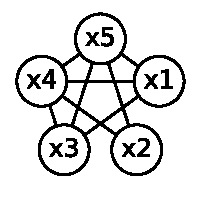
\includegraphics[width=0.625\linewidth]{img/8ec60eeeaa549478379fc4cb6b42df17c5ca8b364e4e642efbba0ac2db0b6e94.pdf}
		\vspace{-1em}
		\captionof{figure}{\centering Graf Terhubung}
		\label{fig:contoh-graf}
	\end{minipage}
	\begin{minipage}{0.4\linewidth}
		\centering
		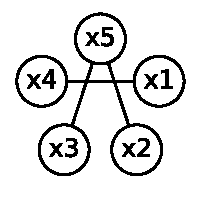
\includegraphics[width=0.625\linewidth]{img/0630ebfe671b8208b2dc56ca90c62464252c4ac5e3f30ff3fc2c6db4495f49cc.pdf}
		\vspace{-1em}
		\captionof{figure}{\centering Graf Tak Terhubung}
		\label{fig:graf-tak-terhubung}
	\end{minipage}
\end{center}

Graf terhubung adalah graf dengan setiap pasang simpulnya memiliki lintasan yang menghubungkan \citep{chartrand2000}. \autoref{fig:contoh-graf} adalah contoh graf terhubung. \autoref{fig:graf-tak-terhubung} adalah contoh graf tak terhubung karena tidak terdapat lintasan yang dapat menghubungkan \(x_1\) dan \(x_5\).

Jarak antara dua simpul \(u\) dan \(v\), dinotasikan \(d(u, v)\), adalah panjang minimum dari semua lintasan yang menghubungkan kedua simpul tersebut \citep{chartrand2000}. Panjang sebuah lintasan adalah banyaknya sisi yang membangun rangkaian lintasan tersebut. Contoh, pada \autoref{fig:contoh-graf}, nilai dari \(d(x_2, x_1)\) adalah \(2\).

Matriks ketetanggaan adalah alternatif representasi dari graf yang menunjukkan ketetanggaan, atau keberadaan sisi antar simpul \citep{west1996}. Semisalnya sebuah graf memiliki himpunan simpul \(V = \{v_1, v_2, \ldots\}\). Maka, baris dan kolom pertama dalam matriks ketetanggaannya menunjukkan \(v_1\), baris dan kolom kedua menunjukkan \(v_2\), dan seterusnya. Ketika terdapat sisi yang menghubungkan \(v_i\) ke \(v_j\), maka elemen pada baris ke-\(i\) dan kolom ke-\(j\) bernilai \(1\), sedangkan bila tidak terhubung maka bernilai \(0\). Sebagai ilustrasi, berikut adalah matriks ketetanggaan dari \autoref{fig:contoh-graf}.
\[
\left[
\begin{array}{ccccc}
	0 & 0 & 1 & 1 & 1 \\
	0 & 0 & 0 & 1 & 1 \\
	1 & 0 & 0 & 1 & 1 \\
	1 & 1 & 1 & 0 & 1 \\
	1 & 1 & 1 & 1 & 0
\end{array}
\right]
\]
Perhatikan matriks ketetanggaan simetris terhadap diagonal utama ketika graf yang direpresentasikan tak berarah.

Matriks jarak adalah matriks yang memuat jarak antara seluruh pasangan simpul \citep{chartrand2000}. Sehingga, setiap baris ke-\(i\) dan kolom ke-\(j\) berisi nilai jarak dari \(v_i\) ke \(v_j\), seperti berikut:
\[
\left[
\begin{array}{ccc}
	d(v_1, v_1) & d(v_1, v_2) & \cdots \\
	d(v_2, v_1) & d(v_2, v_2) & \cdots \\
	\vdots & \vdots & \ddots
\end{array}
\right]
\]
Dan sebagai gambaran, berikut adalah matriks jarak dari \autoref{fig:contoh-graf}.
\[
\left[
\begin{array}{ccccc}
	0 & 2 & 1 & 1 & 1 \\
	2 & 0 & 2 & 1 & 1 \\
	1 & 2 & 0 & 1 & 1 \\
	1 & 1 & 1 & 0 & 1 \\
	1 & 1 & 1 & 1 & 0
\end{array}
\right]
\]
Dapat diamati, setiap elemen dalam matriks jarak memiliki nilai ketika graf yang direpresentasikan adalah graf terhubung.

\section{Automorfisma Graf}

\noindent
\begin{center}
	\begin{minipage}{0.8\linewidth}
		\begin{minipage}{0.25\linewidth}
			\centering
			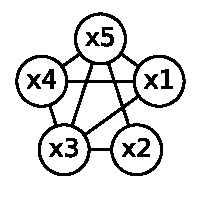
\includegraphics[width=\linewidth]{img/3637d326d230653eb5359219776827aba655cda549265e8622f29fcf4522cfb1.pdf}
			\vspace{-2em}
			\par\small (a)
		\end{minipage}
		\hfill
		\begin{minipage}{0.25\linewidth}
			\centering
			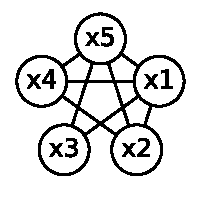
\includegraphics[width=\linewidth]{img/401a2e0bee9ea19714a37a3c2bfa4c78f5a92ea31c623ab3bc7826d5ed95c330.pdf}
			\vspace{-2em}
			\par\small (b)
		\end{minipage}
		\hfill
		\begin{minipage}{0.25\linewidth}
			\centering
			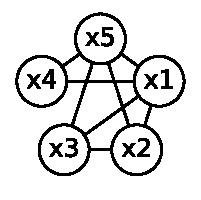
\includegraphics[width=\linewidth]{img/4b541ec99ee9b0f060e784c888fc378dca74b6d8ff80f5ccc8336615aca46695.pdf}
			\vspace{-2em}
			\par\small (c)
		\end{minipage}

		\begin{minipage}{0.25\linewidth}
			\centering
			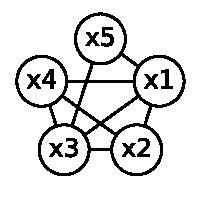
\includegraphics[width=\linewidth]{img/6eeebca324db75f7c0a719672bf306f79b5afe806b2a8814f0b2f2beedb3b891.pdf}
			\vspace{-2em}
			\par\small (d)
		\end{minipage}
		\hfill
		\begin{minipage}{0.25\linewidth}
			\centering
			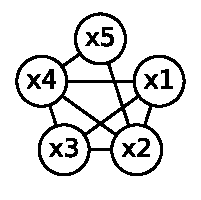
\includegraphics[width=\linewidth]{img/71f4c81555ee6516f44f4d05f5e6f67edd5de0ed42a1cdbcb2f2af72c3232b75.pdf}
			\vspace{-2em}
			\par\small (e)
		\end{minipage}
		\hfill
		\begin{minipage}{0.25\linewidth}
			\centering
			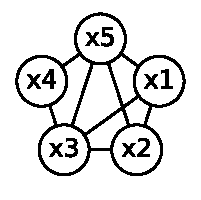
\includegraphics[width=\linewidth]{img/7d7c7231a399fc001d20da820222d60b8205b145c0e4fafd9cf2f3ebf1eec22d.pdf}
			\vspace{-2em}
			\par\small (f)
		\end{minipage}
		\captionof{figure}{Automorfisma Graf}
		\label{fig:contoh-automorfisma}
	\end{minipage}
\end{center}

Automorfisma graf adalah isomorfima suatu graf ke dirinya sendiri. Salah satu cara untuk menunjukkan automorfisma graf adalah menggunakan representasi kanonik. Hal ini telah dilakukan oleh \citeauthor{mckay2014} di \citeyear{mckay2014}. Jika dua graf memiliki representasi kanonik yang sama, maka kedua graf tersebut isomorfik. Sebaliknya, jika representasi kanonik berbeda, maka kedua graf tersebut tidak isomorfik.

Untuk graf tak berarah, representasi kanonik oleh \citeauthor{mckay2014} dituliskan dalam format \verb`graph6`. Sebagai ilustrasi, \autoref{fig:contoh-graf} memiliki representasi \verb`DV{` dalam format \verb`graph6`. Kemudian, setiap graf pada \autoref{fig:contoh-automorfisma}, dari (a) sampai (f), berturut-turut memiliki representasi \verb`D\{`, \verb`Du{`,  \verb`D{{`,  \verb`D~g`,  \verb`D~S`,  dan \verb`Dx{` dalam format \verb`graph6`. Akan tetapi, graf pada \autoref{fig:contoh-graf} dan semua graf pada \autoref{fig:contoh-automorfisma} memiliki representasi kanonik yang sama, yaitu \verb`DN{` dalam format \verb`graph6`, sehingga semuanya merupakan automorfisma dari graf yang sama.

\section{Dimensi Metrik}

Misalkan \(G\) adalah sebuah graf terhubung dengan himpunan simpul \(V = \{v_1, v_2, \ldots, v_n\}\), dan \(d(x, y)\) adalah jarak antara simpul \(x\) dan \(y\) di \(G\). Pilih sembarang \(W = \{w_1, w_2, \ldots, w_k\} \subseteq V\). Untuk \(v \in V\), tupel terurut
	\[ r(v|W) = (d(w_1, v), d(w_2, v), \ldots, d(w_k, v)) \]
adalah representasi dari \(v\) terhadap \(W\). Himpunan \(W\) adalah \foreign{resolving set}, atau himpunan pembeda, untuk \(G\) apabila
	\[ \forall u, v \in V, u \neq v \implies r(u|W) \neq r(v|W) \]
atau dengan kata lain, seluruh simpul dalam \(G\) memiliki representasi unik terhadap \(W\).

Dimensi metrik dari \(G\) adalah kardinalitas minimum dari himpunan pembeda untuk \(G\) \citep{tillquist2023}. Sebagai ilustrasi, ambil \autoref{fig:contoh-graf}. Coba \(W = \{x_2, x_4\}\).
\[
\begin{array}{ccccc}
	r(x_1|W) & = & ( d(x_2, x_1), \; d(x_4, x_1) ) & = & (2, 1) \\
	r(x_2|W) & = & ( d(x_2, x_2), \; d(x_4, x_2) ) & = & (0, 1) \\
	r(x_3|W) & = & ( d(x_2, x_3), \; d(x_4, x_3) ) & = & (2, 1) \\
	r(x_4|W) & = & ( d(x_2, x_4), \; d(x_4, x_4) ) & = & (1, 0) \\
	r(x_5|W) & = & ( d(x_2, x_5), \; d(x_4, x_5) ) & = & (1, 1)
\end{array}
\]
Ditemukan \(\{x_2, x_4\}\) bukanlah himpunan pembeda karena \(r(x_1|W) = r(x_3|W)\). Untuk \autoref{fig:contoh-graf}, tidak ada himpunan pembeda dengan kardinalitas 2. Dimensi metrik dari graf ini adalah 3, dengan contoh solusi \(\{x_1, x_4, x_5\}\), atau \(\{x_1, x_3, x_4\}\), dan himpunan pembeda lainnya yang berkardinalitas 3.

\section{Dimensi Metrik Sisi}

Misalkan \(G\) adalah sebuah graf terhubung dengan himpunan simpul \(V\), himpunan sisi \(E = \{e_1, e_2, \ldots, e_n\}\), dan \(d(x, y)\) adalah jarak antara simpul \(x\) dan \(y\) di \(G\). Untuk sembarang simpul \(z\) dan sembarang sisi \(e\) di \(G\), jika \(e\) adalah sisi yang menghubungkan simpul \(x\) dan \(y\), maka jarak dari \(z\) ke \(e\) adalah \( d(z, e) = \min(d(z, x), d(z, y)) \). Ambil sembarang \(W = \{w_1, w_2, \ldots, w_k\} \subseteq V\). Untuk \(e \in E\), tupel terurut
	\[ r(e|W) = (d(w_1, e), d(w_2, e), \ldots, d(w_k, e)) \]
adalah representasi dari \(e\) terhadap \(W\). Himpunan \(W\) adalah \foreign{edge resolving set}, atau himpunan pembeda sisi, untuk \(G\) apabila
	\[ \forall e, f \in E, e \neq f \implies r(e|W) \neq r(f|W) \]
atau dengan kata lain, seluruh sisi dalam \(G\) memiliki representasi unik terhadap \(W\).

Dimensi metrik sisi dari \(G\) adalah kardinalitas minimum dari himpunan pembeda sisi untuk \(G\) \citep{kelenc2018}. Sebagai ilustrasi, ambil \autoref{fig:contoh-graf}. Coba \(W = \{x_1, x_4, x_5\}\).
\[
\begin{array}{ccccc}
	r(e_1|W) & = & ( d(x_1, e_1), \; d(x_4, e_1), \; d(x_5, e_1) ) & = & (0, 1, 1) \\
	r(e_2|W) & = & ( d(x_1, e_2), \; d(x_4, e_2), \; d(x_5, e_2) ) & = & (0, 0, 1) \\
	r(e_3|W) & = & ( d(x_1, e_3), \; d(x_4, e_3), \; d(x_5, e_3) ) & = & (0, 1, 0) \\
	r(e_4|W) & = & ( d(x_1, e_4), \; d(x_4, e_4), \; d(x_5, e_4) ) & = & (1, 0, 1) \\
	r(e_5|W) & = & ( d(x_1, e_5), \; d(x_4, e_5), \; d(x_5, e_5) ) & = & (1, 1, 0) \\
	r(e_6|W) & = & ( d(x_1, e_6), \; d(x_4, e_6), \; d(x_5, e_6) ) & = & (1, 0, 1) \\
	r(e_7|W) & = & ( d(x_1, e_7), \; d(x_4, e_7), \; d(x_5, e_7) ) & = & (1, 1, 0) \\
	r(e_8|W) & = & ( d(x_1, e_8), \; d(x_4, e_8), \; d(x_5, e_8) ) & = & (1, 0, 0)
\end{array}
\]
Ditemukan \(\{x_1, x_4, x_5\}\) bukanlah himpunan pembeda sisi karena \(r(e_4|W) = r(e_6|W)\). Untuk \autoref{fig:contoh-graf}, tidak ada himpunan pembeda sisi dengan kardinalitas 3. Dimensi metrik sisi dari graf ini adalah 4, dengan contoh solusi \(\{x_1, x_2, x_3, x_4\}\), atau \(\{x_1, x_2, x_3, x_5\}\), dan himpunan pembeda sisi lainnya yang berkardinalitas 4.

\section{\foreign{Satisfiability Modulo Theories}}

SMT, atau \foreign{satisfiability modulo theories}, secara umum adalah proses mencari nilai dari variabel-variabel dalam ekspresi matematika yang menyebabkan ekspresi tersebut menjadi benar. Jika suatu solusi ada, ekspresi tersebut terbilang \foreign{satisfiable}. Jika solusi tidak ada, ekspresi tersebut terbilang \foreign{unsatisfiable}. Proses ini tidak menentukan solusi mana yang akan diberikan, melainkan hanya mencari satu solusi apa pun, yang kemudian disebut sebagai \foreign{model}.

Istilah \foreign{modulo theories} merujuk pada penggunaan teori tertentu, seperti aritmetika bilangan bulat, bilangan riil, \foreign{array}, atau \foreign{bit-vectors}. Pemilihan teori biasanya disesuaikan dengan tujuan pemodelan. Bergantung pada apakah suatu permasalahan ingin ditunjukkan sebagai \foreign{satisfiable} atau \foreign{unsatisfiable}, teori yang digunakan dapat pula berbeda untuk memfasilitasi pemanfaatan sifat-sifat permasalahan tersebut agar lebih ramah terhadap komputasi.

\foreign{Solver} adalah program yang mengimplementasikan proses dari SMT, mengevaluasi ekspresi, dan dapat menghasilkan model. Secara komputasi, \foreign{solver} mungkin untuk tidak menunjukkan hasil, bergantung pada konfigurasi seperti batas waktu eksekusi, maupun dari keterbatasan implementasi teori.

Penjelasan lebih lengkap mengenai SMT dapat ditemukan pada \cite{barrett2018}.

\subsection{\foreign{Boolean Satisfiability}}

\foreign{Boolean satisfiability} dalam SMT adalah teori yang memuat variabel boolean dan operasi boolean pada umumnya \citep{yurichev}. Sebagai ilustrasi, dapat diperhatikan ekspresi
	\[ (x_1 \land x_2) \lor (x_1 \land x_3) \]
dengan \(x_1, x_2, x_3\) adalah variabel boolean. Tabel kebenaran untuk ekspresi tersebut dapat dikonstruksi seperti berikut:
\vspace{-0.5em}
\[
\begin{array}{cccc}
	x_1 & x_2 & x_3 & (x_1 \land x_2) \lor (x_1 \land x_3) \\ [4pt]
	\False & \False & \False & \False \\
	 \True & \False & \False & \False \\
	\False &  \True & \False & \False \\
	 \True &  \True & \False &  \True \\
	\False & \False &  \True & \False \\
	 \True & \False &  \True &  \True \\
	\False &  \True &  \True & \False \\
	 \True &  \True &  \True &  \True
\end{array}
\]

\noindent Oleh karena itu, salah satu \foreign{model} yang dapat dihasilkan oleh \foreign{solver} adalah \(x_1 = \True, x_2 = \False, x_3 = \True\).

Dalam \foreign{boolean satisfiability}, terdapat pula batasan \(\mathrm{AtLeast}\) dan \(\mathrm{AtMost}\) untuk menentukan paling sedikit dan paling banyak variabel yang boleh bernilai benar. Misalnya, dengan menambahkan batasan \(\mathrm{AtLeast}(3)\) ke contoh sebelumnya, \(x_1 = \True, x_2 = \False, x_3 = \True\) tidaklah lagi solusi yang sah.

\subsection{\foreign{Pseudo Boolean}}

\foreign{Pseudo boolean} adalah ekstensi dari teori \foreign{boolean satisfiability} yang dapat menyatakan bentuk ekspresi linear dengan koefisien bilangan bulat atas variabel boolean \citep{yurichev}. Teori ini mendukung tiga operasi relasi, yaitu:
\[
\begin{array}{lcl}
	a_1 x_1 + a_2 x_2 + \ldots + a_i x_i &\leq& a \\
	b_1 x_1 + b_2 x_2 + \ldots + b_j x_j &=& b \\
	c_1 x_1 + c_2 x_2 + \ldots + c_k x_k &\geq& c \\
\end{array}
\]
di mana \(a, a_1, \ldots, a_i, b, b_1, \ldots, b_j, c, c_1, \ldots, c_k\) adalah konstanta \foreign{integer} (bilangan bulat), dan \(x_1,\ldots,x_i,x_j,x_k\) adalah variabel boolean. Ketika variabel boolean bernilai benar, perkaliannya dengan konstanta menjadi seperti perkalian dengan angka 1. Ketika variabel boolean bernilai salah, perkaliannya dengan konstanta menjadi seperti perkalian dengan angka 0. Ambil contoh berikut:
\[
\begin{array}{rcl}
	x_1 + x_2 + x_3 + x_4 &=& 2 \\
	x_1 + x_2 &\leq& 1 \\
	x_3 + x_4 &\leq& 1
\end{array}
\]
dengan \(x_1, x_2, x_3, x_4\) adalah variabel boolean. Ekspresi ini memiliki seluruh konstantanya yang sama dengan 1. Salah satu \foreign{model} yang dapat dihasilkan oleh \foreign{solver} adalah \(x_1 = \True, x_2 = \False, x_3 = \True, x_4 = \False\).

\subsection{\foreign{Linear Integer Arithmetic}}

\foreign{Linear integer arithmetic}, atau LIA, dalam SMT adalah teori yang memuat variabel \foreign{integer}, atau bilangan bulat, dan operasi \foreign{integer} pada umumnya \citep{yurichev}. Contoh \foreign{pseudo boolean} sebelumnya dapat dinyatakan ulang dalam bentuk LIA.
\[
\begin{array}{rcl}
	x_1 + x_2 + x_3 + x_4 &=& 2 \\
	x_1 + x_2 &\leq& 1 \\
	x_3 + x_4 &\leq& 1
\end{array}
\]
\[ 0 \leq x_1 \leq 1, \quad 0 \leq x_2 \leq 1, \quad 0 \leq x_3 \leq 1, \quad 0 \leq x_4 \leq 1 \]
dengan \(x_1, x_2, x_3, x_4\) adalah variabel \foreign{integer}. \foreign{Model} yang dapat dihasilkan oleh \foreign{solver} yang mirip dengan hasil dari \foreign{pseudo boolean} sebelumnya adalah \(x_1 = 1, x_2 = 0, x_3 = 1, x_4 = 0\).

\section{Z3}

Z3 adalah salah satu dari banyak \foreign{solver} SMT yang ada. Z3 dikembangkan oleh Microsoft Research dan dirancang khusus untuk menyelesaikan formula logika dari berbagai macam jenis teori. Z3 merupakan \foreign{solver} modular, dengan menggunakan arsitektur DPLL(T), menggabungkan berbagai prosedur untuk teori-teori yang berbeda \citep{demoura2008}.

Dibandingkan dengan \foreign{solver} lain yang hanya mengkhususkan diri pada teori-teori tertentu, Z3 mendukung kombinasi teori yang lebih kompleks . Selain itu, Z3 juga mendukung penyelesaian inkremental, generasi bukti (\foreign{proof generation}), ekstraksi \foreign{unsat core}, serta penggunaan kuantor (universal dan eksistensial) \citep{bjorner}.

Perlu dipahami bahwa Z3, maupun SMT \foreign{solver} pada umumnya, tidak melakukan manipulasi simbolik sebagaimana \foreign{computer algebra system} (CAS). SMT \foreign{solver} difokuskan pada penentuan \foreign{satifiability} suatu ekspresi menggunakan prosedur seperti DPLL(T) \citep{demoura2008, bjorner}. Sebaliknya, CAS dirancang untuk manipulasi simbolik seperti penyederhanaan ekspresi, integrasi, atau diferensiasi simbolik \citep{geddes1992}. Oleh karena itu, SMT \foreign{solver} dan CAS merupakan kelas asisten komputasi yang berbeda.

\clearpage

\newcommand{\mcol}[3]{\multicolumn{#1}{#2}{#3}}
\newcommand{\mrow}[2]{\multirow{#1}{*}{#2}}
\newcommand{\cellb}{\cellcolor[HTML]{000000}}

\chapter{Metodologi}

Metodologi yang digunakan dalam tugas akhir ini dirancang untuk menyusun, mengimplementasikan, dan mengevaluasi pendekatan berbasis SMT dalam menghitung dimensi metrik dan dimensi metrik sisi suatu graf. Tahapan metodologi ini dibagi menjadi beberapa bagian sebagaimana diilustrasikan oleh \autoref{fig:diagram-alir}.

\begin{figure}[!htbp]
	\centering
	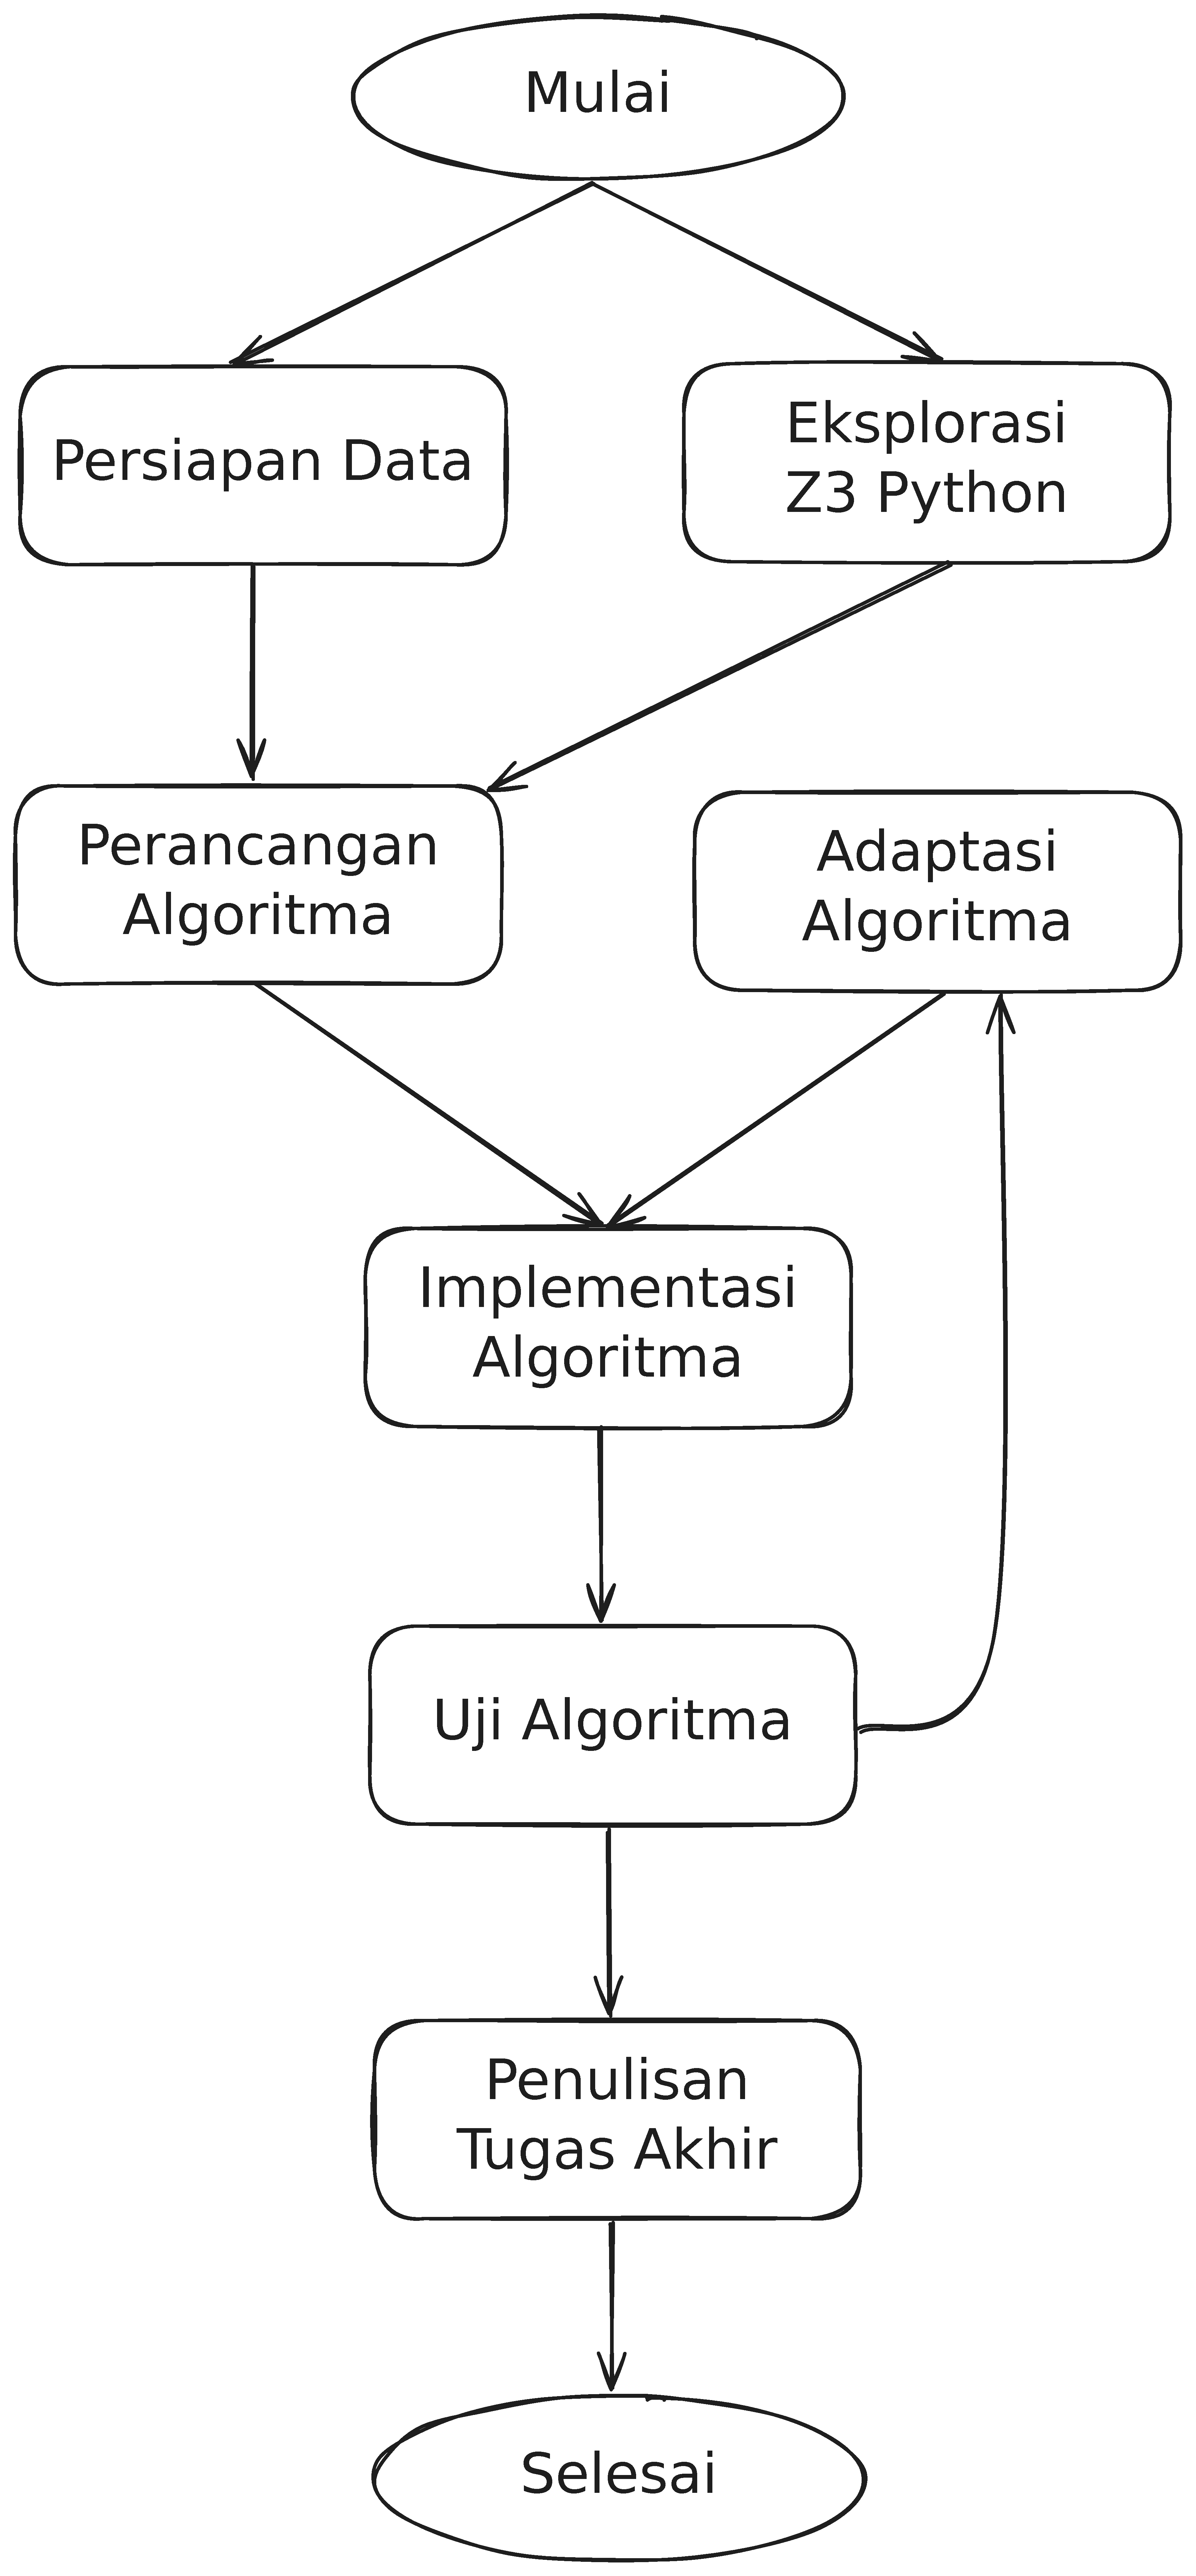
\includegraphics[width=0.5\linewidth]{img/diagram-alir-metodologi.pdf}
	\caption{Diagram Alir Metodologi}
	\label{fig:diagram-alir}
\end{figure}

\clearpage
\section{Persiapan Data}
\label{sec:data}

Data graf yang digunakan dibagi menjadi dua kategori: graf kecil (2 hingga 9 simpul) dan graf besar (lebih dari 9 simpul).

\begin{enumerate}

	\item Graf Kecil

	Graf tak berarah dengan banyak simpul 2 hingga 9 digenerasikan menggunakan program \verb`nauty-geng`. Program ini menghasilkan seluruh graf dengan banyak simpul yang dispesifikasikan dan juga mengeliminasi semua redundansi automorfimanya. Opsi \verb`-c` diberikan kepada program untuk memastikan hanya graf terhubung yang dihasilkan.

	\item Graf Besar

	Graf besar digenerasikan secara acak menggunakan program \verb`nauty-genrang`. Opsi \verb`-g` diberikan kepada program untuk memastikan hanya graf tak berarah yang dihasilkan. Untuk menghindari duplikasi akibat automorfisma, setiap graf diproses menggunakan program \verb`nauty-labelg` untuk menghasilkan representasi kanonik. Kemudian, program \verb`nauty-pickg` dengan opsi \verb`-vc0` digunakan untuk memilih hanya graf yang terkoneksi.

\end{enumerate}

Semua graf disimpan dalam \foreign{file} teks menggunakan format \verb`graph6`. Graf dengan banyak simpul yang sama disimpan dalam file yang sama.

Banyak simpul maksimum yang dapat diuji bergantung pada keterbatasan waktu dan sumber daya komputasi yang tersedia.

\section{Eksplorasi Z3 Python}

Pada tahap ini dilakukan eksplorasi SMT \foreign{solver}, yaitu Z3, menggunakan \foreign{binding} untuk bahasa Python. Aktivitas meliputi:

\begin{enumerate}

	\item Mempelajari fitur dasar Z3 yang relevan dengan formulasi masalah kombinatorial pada teori graf.

	\item Mencoba contoh sederhana untuk memahami cara mendefinisikan variabel, batasan (\foreign{constraints}), serta strategi pencarian solusi.

	\item Mengevaluasi kemampuan Z3 dalam menangani permasalahan berukuran kecil maupun besar untuk mengidentifikasi potensi kendala performa.

\end{enumerate}

\section{Perancangan Algoritma}

Perancangan algoritma difokuskan pada formulasi masalah dimensi metrik ke dalam bentuk SMT. Pertama, graf direpresentasikan dalam bentuk matriks ketetanggaan yang dibaca dari format \verb`graph6`. Kedua, matriks jarak dapat dibangun dari matriks ketetanggaan menggunakan algoritma \foreign{Floyd–Warshall}. Kemudian, berdasarkan dua informasi ini, dirancanglah algoritma yang memetakan pencarian dimensi metrik ke dalam bentuk batasan yang dapat dicerna oleh SMT.

\section{Implementasi Algoritma}

Algoritma yang telah dirancang kemudian diimplementasikan ke bentuk kode. Hal-hal yang perlu dilakukan diantaranya adalah:

\begin{enumerate}

		\item Pembacaan graf dari \foreign{file} teks \verb`graph6`.

		\item Formulasi batasan untuk SMT dari informasi graf.

		\item Eksekusi Z3 \foreign{solver} dan dapatkan dimensi metrik.

		\item Simpan hasil perhitungan ke dalam \foreign{file} teks untuk analisis lebih lanjut.

\end{enumerate}

\section{Uji Algoritma}

Pengujian dilakukan secara bertahap untuk memverifikasi kebenaran implementasi serta mengevaluasi kinerjanya.

\begin{enumerate}

	\item{Uji pada Sampel Kecil}

	Beberapa graf kecil dipilih sebagai sampel. Tujuan tahap pengujian ini adalah memverifikasi bahwa rancangan algoritma dan implementasi program menghasilkan solusi yang benar.

	\item{Uji pada Seluruh Graf Kecil}

	Seluruh graf terhubung dengan 2–9 simpul diuji secara menyeluruh. Tujuan tahap pengujian ini adalah untuk mendapatkan data komprehensif kinerja algoritma dengan berbagai macam konfigurasi graf. Data ini dapat dianalisis kasus-kasusnya seperti kejadian \foreign{worst-case} dan kejadian \foreign{best-case}. Hasil ini juga dapat dibandingkan dengan literatur yang ada untuk validasi.

	\item{Uji pada Graf Besar}

	Pengujian diperluas pada graf dengan simpul lebih banyak. Tujuan tahap pengujian ini adalah mengevaluasi kinerja dan keterbatasan pendekatan SMT pada kasus yang lebih kompleks. Uji ini juga yang dijadikan sebagai tolak ukur performa solusi dari tugas akhir ini secara umum untuk sembarang graf.

\end{enumerate}

\section{Adaptasi Algoritma}

Tahap adaptasi dilakukan dengan memodifikasi algoritma yang telah ada untuk menghitung dimensi metrik sisi. Proses adaptasi mencakup:

\begin{enumerate}

	\item Menyesuaikan representasi graf sehingga memperhatikan jarak antar sisi.

	\item Memformulasikan kembali permasalahan ke dalam SMT.

	\item Mengimplementasikan kembali ke bentuk kode.

	\item Mengulangi tahapan pengujian: mulai dari sampel kecil, seluruh graf kecil, hingga graf besar.

\end{enumerate}

\section{Penulisan Tugas Akhir}

Tahap terakhir dari metodologi ini adalah penyusunan seluruh hasil penelitian ke dalam bentuk laporan tugas akhir. Penulisan dilakukan sesuai pedoman akademik yang berlaku sehingga hasil penelitian terdokumentasi dengan baik dan dapat dijadikan rujukan untuk penelitian selanjutnya.

\section{Jadwal Kegiatan}

Jadwal kegiatan pada \autoref{tab:jadwal-kegiatan} disusun untuk memberikan gambaran alur waktu pelaksanaan tugas akhir.

\begin{table}[!htbp]
	\centering
	\caption{Jadwal Kegiatan}
	\begin{tabular}{|c|l|llllllllllll|}
		\hline
		 &  & \mcol{12}{c|}{Minggu} \\ \cline{3-14}
		\mrow{-2}{No} & \mrow{-2}{Nama Kegiatan} & \mcol{1}{c|}{1} & \mcol{1}{l|}{2} & \mcol{1}{l|}{3} & \mcol{1}{l|}{4} & \mcol{1}{l|}{5} & \mcol{1}{l|}{6} & \mcol{1}{l|}{7} & \mcol{1}{l|}{8} & \mcol{1}{l|}{9} & \mcol{1}{l|}{10} & \mcol{1}{l|}{11} & 12 \\ \hline
		1 & Persiapan Data & \mcol{1}{c|}{\cellb} & \mcol{1}{l|}{\cellb} & \mcol{1}{l|}{} & \mcol{1}{l|}{} & \mcol{1}{l|}{} & \mcol{1}{l|}{} & \mcol{1}{l|}{} & \mcol{1}{l|}{} & \mcol{1}{l|}{} & \mcol{1}{l|}{} & \mcol{1}{l|}{} &  \\ \hline
		2 & Eksplorasi Z3 Python & \mcol{1}{c|}{\cellb} & \mcol{1}{l|}{\cellb} & \mcol{1}{l|}{} & \mcol{1}{l|}{} & \mcol{1}{l|}{} & \mcol{1}{l|}{} & \mcol{1}{l|}{} & \mcol{1}{l|}{} & \mcol{1}{l|}{} & \mcol{1}{l|}{} & \mcol{1}{l|}{} &  \\ \hline
		3 & Perancangan Algoritma & \mcol{1}{l|}{} & \mcol{1}{l|}{\cellb} & \mcol{1}{l|}{\cellb} & \mcol{1}{l|}{} & \mcol{1}{l|}{} & \mcol{1}{l|}{} & \mcol{1}{l|}{} & \mcol{1}{l|}{} & \mcol{1}{l|}{} & \mcol{1}{l|}{} & \mcol{1}{l|}{} &  \\ \hline
		4 & Implementasi Algoritma & \mcol{1}{l|}{} & \mcol{1}{l|}{} & \mcol{1}{l|}{\cellb} & \mcol{1}{l|}{\cellb} & \mcol{1}{l|}{} & \mcol{1}{l|}{} & \mcol{1}{l|}{} & \mcol{1}{l|}{} & \mcol{1}{l|}{} & \mcol{1}{l|}{} & \mcol{1}{l|}{} &  \\ \hline
		5 & Uji Algoritma & \mcol{1}{l|}{} & \mcol{1}{l|}{} & \mcol{1}{l|}{} & \mcol{1}{l|}{\cellb} & \mcol{1}{l|}{\cellb} & \mcol{1}{l|}{\cellb} & \mcol{1}{l|}{} & \mcol{1}{l|}{\cellb} & \mcol{1}{l|}{\cellb} & \mcol{1}{l|}{\cellb} & \mcol{1}{l|}{} &  \\ \hline
		6 & Adaptasi Algoritma & \mcol{1}{l|}{} & \mcol{1}{l|}{} & \mcol{1}{l|}{} & \mcol{1}{l|}{} & \mcol{1}{l|}{} & \mcol{1}{l|}{\cellb} & \mcol{1}{l|}{\cellb} & \mcol{1}{l|}{\cellb} & \mcol{1}{l|}{} & \mcol{1}{l|}{} & \mcol{1}{l|}{} &  \\ \hline
		7 & Penulisan Tugas Akhir & \mcol{1}{l|}{} & \mcol{1}{l|}{} & \mcol{1}{l|}{} & \mcol{1}{l|}{} & \mcol{1}{l|}{} & \mcol{1}{l|}{} & \mcol{1}{l|}{} & \mcol{1}{l|}{} & \mcol{1}{l|}{} & \mcol{1}{l|}{} & \mcol{1}{l|}{\cellb} & \cellb \\ \hline
	\end{tabular}
	\label{tab:jadwal-kegiatan}
\end{table}

Jadwal kegiatan membantu membatasi waktu setiap tahap agar penelitian dapat berjalan sesuai rencana. Tabel ini juga berfungsi sebagai acuan untuk memantau kemajuan dan menyesuaikan perkembangan bila ada keterlambatan.

\clearpage

%! TEX root = self_chapter-4.tex

\setcounter{chapter}{3}
\chapter{Hasil dan Pembahasan}

\def\True{\mathtt{True}}
\def\False{\mathtt{False}}
\def\min{\mathtt{min}}
\def\Bbb{\mathbb{B}}
\renewcommand{\foreign}[1]{\foreignlanguage{english}{\textit{#1}}}

\section{Landasan Formal}

Untuk mempermudah pembahasan, terlebih dahulu didefinisikan beberapa notasi. Misalkan \(S\) merupakan suatu himpunan sembarang. Sebuah vektor berdimensi \(n\) yang elemennya berasal dari \(S\) ditulis sebagai \(c \in S^n\), dengan \(c_i \in S\) menyatakan elemen ke-\(i\) dari vektor tersebut. Vektor \(c\) dapat dibangun dari elemen-elemennya dengan notasi \(c = (c_1\ \cdots\ c_n)\), atau secara singkat \(c = (c_i\ \cdots)\) ketika domain indeks \(i\) jelas dari konteks.

Selanjutnya, sebuah matriks \(A\) berukuran \(m\) baris dan \(n\) kolom yang elemennya berasal dari \(S\) ditulis sebagai \(A \in S^{m\times n}\), dengan \(A_{ij} \in S\) menyatakan elemen di baris ke-\(i\) dan kolom ke-\(j\) dari matriks tersebut. Digunakan notasi \(A_{*j} \in S^m\) untuk kolom ke-\(j\) dan \(A_{i*} \in S^n\) untuk baris ke-\(i\).

Kemudian, misalnya, diberikan \(a_1,\ \cdots,\ a_m \in S^n\). Sebuah matriks \(A \in S^{n\times m}\) dapat dibangun dengan menyusun vektor-vektor tersebut secara bersampingan, yaitu \(A = [a_1\ \cdots\ a_m]\), atau secara singkat \(A = [a_i\ \cdots]\) ketika domain indeks \(i\) jelas dari konteks. Demikian pula, sebuah matriks \(A \in S^{m\times n}\) dapat dibangun dengan menyusun vektor-vektor tersebut secara bertumpuk, yaitu
	\[ A = \left[ \begin{array}{c} a_1\\ \vdots\\ a_m \end{array} \right], \quad \text{atau secara singkat } A = \left[ \begin{array}{c} a_i\\ \vdots \end{array} \right] \text{.}\]

Dengan demikian, matriks \(A\) dapat dibangun dari elemen-elemen barisnya maupun dari elemen-elemen kolomnya sebagai berikut.
	\[ A = \left[ \begin{array}{c} A_{i*}\\ \vdots \end{array} \right] = [A_{*j}\ \cdots] \]

Selanjutnya, didefinisikan sebuah operator boolean biner sebagai operasi yang memetakan dua unsur ke dalam nilai boolean \(\Bbb = \{\True, \False\}\). Untuk setiap \(s_1, s_2 \in S\), didefinisikan \((s_1 = s_2) \in \Bbb\) sebagai berikut.
	\[ (s_1 = s_2) = \left\{
	\begin{array}{l@{\ }l}
		\True  &\iff s_1 = s_2 \\
		\False &\iff s_1 \neq s_2
	\end{array} \right. \]
Secara natural, operator tersebut dapat diperluas untuk \(a, b \in S^n\), sehingga \((a = b) \in \Bbb^n\) merupakan vektor boolean yang komponennya diberikan oleh \((a = b)_i = (a_i = b_i)\), dan oleh karena itu \((a = b) = ((a_i = b_i)\ \cdots)\).

\cleardoublepage

Didefinisikan sebuah operator boolean biner lain yang berbentuk \((s_1 | s_2) \in \Bbb\) untuk \(s_1, s_2 \in S\) sebagai berikut.
	\[ (s_1 = s_2) = \left\{
	\begin{array}{l@{\ }l@{\ }c}
		\True  &\iff& s_1 \vee s_2 \\
		\False &\iff& \neg s_1 \wedge \neg s_2
	\end{array} \right. \]
Seperti sebelumnya, operator ini diperluas untuk \(a, b \in S^n\) dengan \((a | b) = ((a_i | b_i)\ \cdots) \in \Bbb^n\).

Terakhir, diperkenalkan beberapa notasi yang berhubungan dengan graf. Misalkan \(G\) adalah graf. Representasi graf \(G\) dalam bentuk matriks ketetanggaan ditulis sebagai \(M\). Untuk \(V\), himpunan seluruh simpul di \(G\), matriks jarak simpul ke simpul dari \(G\) ditulis sebagai \(D^{(V)}\), sehingga jarak antar dua simpul \(v_i,v_j \in V\) adalah \(d(v_i,v_j) = D_{i,j}^{(V)}\). Untuk \(E\), himpunan seluruh sisi di \(G\), matriks jarak simpul ke sisi dari \(G\) ditulis sebagai \(D^{(E)}\), sehingga jarak antara simpul \(v_i \in V\) dan sisi \(e_j \in E\) adalah \(d(v_i,e_j) = D_{i,j}^{(E)}\).

Dengan menggunakan notasi yang telah didefinikan, perhatikan bahwa matriks jarak simpul ke simpul dapat dibangun melalui representasi, yaitu \(D = [r(v_i|V)\ \cdots]\), karena \(r(u|V) = (d(u,v_j)\ \cdots), v_j \in V\). Demikian pula, matriks jarak simpul ke sisi dapat dibangun melalui representasi, yaitu \(D = [r(e_i|V)\ \cdots]\), karena \(r(e,v_j) = (d(e,v_j)\ \cdots), v_j \in V\).

\section{Formulasi Algoritma}

Pondasi yang digunakan oleh seluruh formulasi algoritma di sini adalah matriks yang bernama \foreign{distance similarity matrix} untuk penentuan dimensi metrik, atau \foreign{edge distance similarity matrix} untuk penentuan dimensi metrik sisi. Untuk membangun masing-masing matriks tersebut, diperlukan matriks jarak simpul ke simpul dan matriks jarak simpul ke sisi.

Oleh karena itu, \foreign{input} yang digunakan adalah representasi matriks ketetanggaan \(M\) dari graf \(G\). Kemudian, \(D^{(V)}\) dapat dikonstruksi dari \(M\) menggunakan algoritma \foreign{Floyd-Warshall}. Dan \(D^{(E)}\) dapat dikonstruksi langsung dari definisi jarak simpul ke sisi; yaitu jarak dari simpul \(v_i \in V\) ke sisi \(e_j \in E\), di mana \(e_j\) adalah sisi yang menghubungkan dua simpul \(v_k, v_l \in V\), adalah \(d(v_i,e_j) = \min(d(v_i, v_k), d(v_i, v_l))\), sehingga \(D_{ij}^{(E)} = \min(D_{ik}^{(V)}, D_{il}^{(V)})\).

\foreign{Distance similarity matrix} dari \(G\) yang dinotasikan \(B^{(V)} \in \Bbb^{|V|\times \frac{|V|(|V|-1)}{2}}\) dan \foreign{edge distance similarity matrix} dari \(G\) yang dinotasikan \(B^{(E)} \in \Bbb^{|V|\times \frac{|E|(|E|-1)}{2}}\) berturut-turut merupakan hasil dari perbandingan antara setiap kolom berbeda di \(D^{(V)}\) serta \(D^{(E)}\).
	\[ B^{(V)} = [(D_{*j}^{(V)} = D_{*k}^{(V)})\ \cdots], \quad j < k\]
	\[ B^{(E)} = [(D_{*j}^{(E)} = D_{*k}^{(E)})\ \cdots], \quad j < k\]

Kemudian, dari \(B^{(V)}\), dikonstruksi matriks yang bernama \foreign{reduced distance similarity}, dan dinotasikan \(P^{(V)}\), atau dari \(B^{(E)}\), dikonstruksi matriks yang bernama \foreign{reduced edge distance similarity}, dan dinotasikan \(P^{(E)}\), menggunakan algoritma berikut.
\begin{enumerate}
	\item Tetapkan \(P := B\).
	\item Untuk setiap \(P_{*j}\) dan \(P_{*k}\) dan \(j \neq k\), hapus \(P_{*j}\) jika \((P_{*j} | P_{*k}) = P_{*k}\).
\end{enumerate}

\cleardoublepage

Sebagai contoh, perhatikan graf berikut.

\begin{figure}[!htbp]
	\centering
	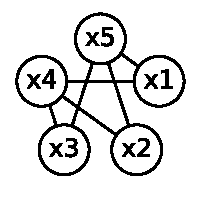
\includegraphics[width=0.25\linewidth]{img/f372738d3845db182fe0b4a3eced9bc2ac778c82a1804f5788cce6bb74ea1beb.pdf}
	\caption{Contoh Graf}
	\label{fig:contoh-graf}
\end{figure}

Graf ini memiliki representasi dalam matriks ketetanggaan sebagai berikut.
\[
	M = \left[ \begin{array}{ccccc}
		0 & 0 & 0 & 1 & 1 \\
		0 & 0 & 0 & 1 & 1 \\
		0 & 0 & 0 & 1 & 1 \\
		1 & 1 & 1 & 0 & 0 \\
		1 & 1 & 1 & 0 & 0
	\end{array} \right]
\]

Menggunakan \foreign{Floyd-Warshall}, didapatkan matriks jarak simpul ke simpul berikut.
\[
	D^{(V)} = \left[ \begin{array}{ccccc}
		0 & 2 & 2 & 1 & 1 \\
		2 & 0 & 2 & 1 & 1 \\
		2 & 2 & 0 & 1 & 1 \\
		1 & 1 & 1 & 0 & 2 \\
		1 & 1 & 1 & 2 & 0
	\end{array} \right]
\]

Selanjutnya, dihasilkan \foreign{distance similarity matrix} berikut.
\[
	B^{(V)} = \left[ \begin{array}{cccccccccc}
		\False & \False & \False & \False &  \True & \False & \False & \False & \False &  \True \\
		\False &  \True & \False & \False & \False & \False & \False & \False & \False &  \True \\
		 \True & \False & \False & \False & \False & \False & \False & \False & \False &  \True \\
		 \True &  \True & \False & \False &  \True & \False & \False & \False & \False & \False \\
		 \True &  \True & \False & \False &  \True & \False & \False & \False & \False & \False
	\end{array} \right]
\]

Kemudian, setelah penghapusan, didapat \foreign{reduced distance similarity} berikut.

\[
	P^{(V)} = \left[ \begin{array}{ccccc}
		\False & \False & \False &  \True &  \True \\
		\False &  \True & \False & \False &  \True \\
		 \True & \False & \False & \False &  \True \\
		 \True &  \True & \False &  \True & \False \\
		 \True &  \True & \False &  \True & \False \\
	\end{array} \right]
\]

\cleardoublepage

\subsection{\foreign{Brute-force}}

...

\subsection{\foreign{Boolean Satisfiability}}

Minimize the number of \(x_i\) that needs to be \(\True\).
\[
	\begin{array}{rl}
		x_3 \vee x_4 \vee x_5 \implies& x_1 \vee x_2 \\
		x_2 \vee x_4 \vee x_5 \implies& x_1 \vee x_3 \\
		& x_1 \vee x_2 \vee x_3 \vee x_4 \vee x_5 \\
		x_1 \vee x_4 \vee x_5 \implies& x_2 \vee x_3 \\
		x_1 \vee x_2 \vee x_3 \implies& x_4 \vee x_5 \\
	\end{array}
\]

\subsection{\foreign{Linear Integer Arithmetic}}

Minimize \(x_1 + x_2 + x_3 + x_4 + x_5 \).
\[
	\begin{array}{r}
		x_1 + x_2 \geq 1 \\
		x_1 + x_3 \geq 1 \\
		x_1 + x_2 + x_3 + x_4 + x_5 \geq 1 \\
		x_2 + x_3 \geq 1 \\
		x_4 + x_5 \geq 1
	\end{array}
\]

\subsection{\foreign{Pseudo Boolean}}

Minimize \(k\).
\[
	\begin{array}{rl}
		x_1 + x_2 + x_3 + x_4 + x_5 &= k\\ [4pt]
		x_3 + x_4 + x_5 &\leq k - 1 \\
		x_2 + x_4 + x_5 &\leq k - 1 \\
		0 &\leq k - 1 \\
		x_1 + x_4 + x_5 &\leq k - 1 \\
		x_1 + x_2 + x_3 &\leq k - 1
	\end{array}
\]

\section{Evaluasi Algoritma}

\section{Pembahasan}

\clearpage

\chapter{Kesimpulan dan Saran}

\section{Kesimpulan}

Tugas akhir ini bertujuan untuk mempelajari permasalahan penentuan invarian graf berupa dimensi metrik dan dimensi metrik sisi dengan memanfaatkan pendekatan berbasis \foreign{Satisfiability Modulo Theories} (SMT). Fokus tugas akhir ini meliputi hal-hal dari formulasi permasalahan ke dalam bentuk SMT, pengimplementasian formulasi tersebut, hingga evaluasi efektivitas pendekatan yang diusulkan. Berdasarkan hasil yang telah diperoleh, dapat disimpulkan bahwa:

\begin{enumerate}
	\item Permasalahan dimensi metrik dan dimensi metrik sisi dapat direpresentasikan secara sistematis ke dalam bentuk formula SMT, sebagaimana telah didemonstrasikan oleh \autoref{alg:boolean-satisfiability}, \autoref{alg:linear-integer-arithmetic}, dan \autoref{alg:pseudo-boolean}.

	\item Pendekatan SMT dapat digunakan secara praktikal untuk menentukan dimensi metrik maupun dimensi metrik sisi suatu graf. Terlihat dari hasil pada \autoref{sec:implementation} dan tabel-tabel frekuensi pada \autoref{sec:discussion} bahwa strategi tersebut dapat menghasilkan kedua invarian ini dengan benar.

	\item Efektivitas penggunaan SMT dalam menyelesaikan permasalahan dimensi metrik dan dimensi metrik sisi bergantung pada ukuran graf dan sumber daya komputasi yang tersedia, serta pemilihan teori yang digunakan -- seperti yang telah dikaji dalam poin ke-3 pada \autoref{sec:discussion}.
\end{enumerate}

Kesimpulan yang diperoleh dalam tugas akhir ini berlaku dalam batasan-batasan yang telah ditetapkan. Yaitu pemilihan graf yang sederhana, tak berarah, terhubung, dan tak berbobot; banyaknya simpul pada graf yang dibatasi sesuai dengan perencanaan pada \autoref{sec:data}; membatasi waktu eksekusi; serta melakukan eksekusi implementasi menggunakan \foreign{CPU} yang telah dispesifikasikan. Semua hal ini dielaborasikan lebih detail pada \autoref{sec:implementation}. Kebenaran hasil penentuan dimensi metrik atau dimensi metrik sisi menggunakan SMT juga dibantu validasi melalui metode \foreign{brute-force} selama \autoref{alg:brute-force} masih mampu melakukan komputasinya dengan batasan-batasan ini.

Dengan demikian, secara keseluruhan, hasil tugas akhir ini menunjukkan bahwa memetakan suatu perumusan ke dalam SMT merupakan alternatif pendekatan yang layaknya cukup tajam untuk secara sistematis menghadapi permasalahan graf yang relatif rumit, seperti penentuan dimensi metrik dan dimensi metrik sisi.

Diharapkan pekerjaan yang telah dicapai dalam tugas akhir ini berhasil membawa beberapa manfaat. Seperti langkah-langkah analisis yang dilakukan dalam usaha memformulasi permasalahan graf ke dalam SMT diharapkan berkontribusi memberi wawasan baru dalam pengembangan pembelajaran teori graf secara komputasional. Atau cara pemetaan rumusan penentuan dimensi metrik dan dimensi metrik sisi spesifik pada tugas akhir ini yang mungkin menjadi dasar awal untuk pengembangan lebih lanjut. Maupun dokumentasi, implementasi, dan hasil yang diperoleh dapat menjadi referensi bagi tugas akhir atau penelitian selanjutnya dalam teori graf serta bidang ilmu komputer.

\section{Saran}

Banyak aspek dari tugas akhir ini yang masih dapat dikembangkan lebih lanjut. Bagian ini menyajikan beberapa saran sebagai bahan pertimbangan untuk area-area yang dapat dipelajari lebih lanjut. Diskusi saran di sini mencakup aspek lingkup eksperimen, implementasi algoritma, desain algoritma, eksekusi eksperimen, variasi graf, alternatif teori, serta eksplorasi aplikasi.

Secara lingkup eksperimen, batasan-batasan sebagaimana pada \autoref{sec:implementation} dipilih atas pertimbangan praktikalitas pengerjaan dengan waktu dan sumber daya yang tersedia dalam penyusunan tugas akhir ini. Namun, dengan telah selesainya perancangan teori yang mendasari formulasi algoritma-algoritma sebagaimana pada \autoref{sec:alg}, skema eksekusi eksperimen dapat dikembangkan lebih lanjut. Misalnya, evaluasi dapat dilakukan pada graf berukuran lebih besar, mengingat evaluasi pada tugas akhir ini dibatasi hingga 50 simpul. Dengan demikian, batasan waktu eksekusi per iterasi dalam tugas akhir ini yang ditetapkan selama 5 menit dapat diperpanjang untuk mendukung evaluasi graf lebih besar, seiring meningkatnya waktu eksekusi yang cenderung bersifat kombinatorial. Selain itu, interval kenaikan banyak simpul untuk graf besar dapat diperkecil. Dalam tugas akhir ini, interval yang digunakan relatif besar, yaitu 5 simpul. Dengan interval kenaikan simpul lebih kecil, tren seperti pada \autoref{sec:discussion} dapat diperoleh dengan resolusi lebih tinggi, sehingga analisis yang dilakukan dapat menjadi lebih spesifik. Selanjutnya, karena data analisis untuk graf besar pada dasarnya merupakan sampel dari seluruh kemungkinan graf yang ada, maka dapat diambil lebih banyak data. Dalam tugas akhir ini diambil 50 graf sembarang untuk setiap graf bersimpul \(n\); dengan memperbanyak graf yang dievaluasi, karakteristik tabel frekuensi untuk graf besar serta hasil perhitungan rata-rata waktu eksekusi diharapkan dapat menggambarkan variasi antar algoritma yang lebih kaya.

Secara implementasi algoritma, dapat dilakukan modifikasi cara penerapan batasan waktu eksekusi. Pada tugas akhir ini, batas waktu diberikan pada setiap iterasi kardinalitasnya. Hal ini dapat diubah menjadi batasan waktu secara eksekusi total algoritma, yaitu dari awal hingga akhir ditemukannya dimensi metrik ataupun dimensi metrik sisi.

Secara desain algoritma, terdapat tiga arah pengembangan yang dapat dilakukan. Yang paling sederhana adalah aspek perbandingan algoritma terhadap metode \foreign{brute-force}. Dalam tugas akhir ini, desain algoritma \foreign{brute-force} menggunakan landasan teori yang sama dengan algoritma berbasis SMT. Oleh karena itu, artinya metode ini tidak sepenuhnya murni \foreign{brute-force}. Analisis dapat dikembangkan dengan mendesain algoritma \foreign{brute-force} yang lebih \foreign{naive}, dan melihat apakah perbandingan evaluasi terhadap \foreign{brute-force} baru ini menghasilkan kesimpulan yang sama seperti yang ditarik pada \autoref{sec:discussion}. Berikutnya, aspek yang lebih menarik adalah mencoba teori lain dalam SMT, karena tugas akhir ini baru mengeksplorasi pemetaan \foreign{constraint} ke dalam \foreign{boolean satisfiability}, \foreign{linear integer arithmetic}, dan \foreign{pseudo boolean}. Mungkin terdapat teori SMT dengan \foreign{construct} yang lebih tinggi ataupun lebih rendah yang dapat menghasilkan waktu eksekusi lebih cepat, baik untuk graf kecil maupun graf besar. Akhirnya, aspek yang paling menantang untuk dikembangkan adalah mempelajari cara kerja \foreign{conflict driven learning} yang fundamental dalam SMT, dan memformulasi pemetaan yang dapat mengeksploitasi mekanisme ini dengan lebih efektif.

Secara eksekusi eksperimen, terdapat dua pendekatan yang dapat dicoba. Pertama adalah menggunakan \foreign{solver} SMT selain Z3. Kedua adalah menggunakan \foreign{solver} yang memiliki kemampuan \foreign{parallelism}, sehingga dapat memanfaatkan \foreign{multi-core} untuk eksekusi satu individu graf, tanpa mengubah kode implementasi sama sekali. Hasil yang diperoleh dari kedua pendekatan ini kemudian dapat dibandingkan dengan hasil eksekusi klasik menggunakan Z3.

Secara variasi graf, terdapat banyak variasi yang dapat dilakukan. Beberapa contohnya dijelaskan berikut ini. Contoh yang paling jelas adalah dimensi metrik itu sendiri. Tugas akhir ini hanya mengkaji dimensi metrik pada bentuk klasiknya dan dimensi metrik sisi. Beberapa contoh variasi dimensi metrik yang dapat dicoba antara lain adalah \foreign{local metric dimension}, \foreign{mixed metric dimension}, \foreign{k-metric dimension}, \foreign{fault tolerant metric dimension}, \foreign{strong metric dimension}, dan variasi lainnya. Hal lain yang dapat diubah adalah asumsi dalam graf yang digunakan untuk menentukan dimensi metrik itu sendiri. Contohnya, dapat dicoba graf berbobot, atau graf berarah, atau graf tak sederhana, dan sebagainya.

Secara alternatif teori, yang dimaksud adalah pengembangan dari landasan teori fundamental yang telah dikerjakan oleh tugas akhir ini untuk desain setiap algoritmanya, yaitu \foreign{distance similarity matrix}. Pertama, representasi matriks paling optimal ketika graf yang bersangkutan cenderung \foreign{dense}. Sehingga, teori ini dapat dieksplorasi lebih lanjut sifat-sifatnya untuk graf yang cenderung \foreign{sparse}, dan apakah mampu dimodifikasi agar lebih efisien. Kedua, dapat dipelajari lebih lanjut apakah struktur \foreign{distance similarity matrix} ramah untuk melakukan optimasi menggunakan metode \foreign{divide and conquer}, atau apakah matriks ini memiliki struktur yang cukup terkait satu sama lain sehingga menghentikan pendekatan ini. Ketiga, dapat dipelajari apakah pemetaan \foreign{distance similarity matrix} ke \foreign{constraint} dalam SMT mungkin untuk dikonstruksikan sedemikian rupa ramah terhadap paralelisasi. Keempat, eksplorasi teori-teori graf lainnya yang mungkin dapat dimanfaatkan untuk mengambil inferensi dari maupun melakukan transformasi pada \foreign{distance similarity matrix}.

Terakhir, adalah eksplorasi aplikasi. Di luar aplikasi yang telah dibahas pada \autoref{sec:application}, masih banyak lagi potensi penggunaan dimensi metrik yang dapat dieksplorasi, misalnya dalam bidang kimia. Simpul dapat dimodelkan sebagai atom dan sisi sebagai ikatan; dimensi metrik dapat digunakan untuk analisis terkait atom, seperti analisis pola struktural, sedangkan dimensi metrik sisi dapat digunakan untuk analisis terkait ikatan, seperti analisis functional group. Beberapa contoh aplikasinya antara lain adalah:

\begin{enumerate}
	\item Banyak senyawa kimia memiliki komposisi elemen yang sama tetapi struktur berbeda. Dimensi metrik dapat digunakan untuk identifikasi isomer.

	\item Banyak senyawa kimia memiliki derajat kesimetrian yang tinggi, sehingga mereka tampak sama secara lokal. Dimensi metrik sisi dapat digunakan untuk memecah kesimetrian topologi.

	\item Dalam machine learning, biasanya diperlukan data dalam bentuk vektor, sedangkan senyawa kimia biasanya direpresentasikan dalam bentuk simbolik. Dimensi metrik berpotensi berfungsi sebagai encoding yang efektif untuk merepresentasikan senyawa ke dalam representasi vektor.
\end{enumerate}

Secara keseluruhan, saran-saran yang disampaikan pada bagian ini bertujuan untuk membuka peluang pengembangan lebih lanjut. Diharapkan tugas akhir ini dapat menjadi dasar yang lebih kaya untuk studi selanjutnya dalam bidang teori graf dan penerapannya secara komputasional. Segala pengembangan ini diharapkan tidak hanya meningkatkan efektivitas algoritma, tetapi juga memperluas pemahaman dan aplikasi dimensi metrik dalam konteks yang lebih luas.

\clearpage

\backmatter

\appendix

\renewcommand{\thesection}{\Alph{section}}

\chapter{Lampiran}

\section{Implementasi Algoritma}
\label[appsec]{app:code}

\textit{...link to where the code is hosted...}

\section{Data Hasil Eksekusi}
\label[appsec]{app:result}

\textit{...link to where the result is hosted...}

\clearpage

\addcontentsline{toc}{chapter}{Daftar Pustaka}
\bibliographystyle{apalike}
\bibliography{references}
\clearpage

\addcontentsline{toc}{chapter}{Ucapan Terima Kasih}
\chapter*{Ucapan Terima Kasih}

\clearpage

\input{Biography}
\clearpage

\end{document}
